\documentclass[tikz,border=2pt]{standalone}
\usepackage{amsmath}
\usepackage{pgfplots}
\pgfplotsset{compat=1.18}
\usetikzlibrary{arrows.meta}
\begin{document}
% Section 6.2/6.4: initial system [1 -c^T 0 | 0; 0 A I_m | b] becomes the tableau of basis B by
% (1) multiplying the constraint rows by B^{-1}, (2) adding c_B^T times the rows to the objective row:
% [1 -c^T+c_B^T B^{-1}A  c_B^T B^{-1} | c_B^T B^{-1}b; 0 B^{-1}A B^{-1} | B^{-1}b]; slack block I_m -> B^{-1}.
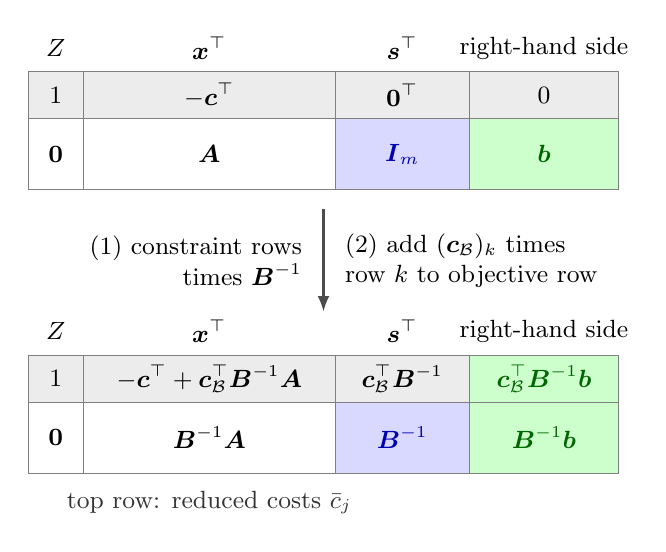
\begin{tikzpicture}[font=\small, >={Latex[length=2mm]}]
  % column boundaries: Z | x | s | RHS
  \def\xa{0}\def\xb{0.7}\def\xc{3.9}\def\xd{5.6}\def\xe{7.5}
  % ---------- initial system ----------
  \begin{scope}
    \fill[gray!15] (\xa,0) rectangle (\xe,-0.6);
    \fill[blue!15] (\xc,-0.6) rectangle (\xd,-1.5);
    \fill[green!20] (\xd,-0.6) rectangle (\xe,-1.5);
    \draw[gray] (\xa,0) rectangle (\xe,-1.5);
    \draw[gray] (\xa,-0.6) -- (\xe,-0.6);
    \foreach \x in {\xb,\xc,\xd} \draw[gray] (\x,0) -- (\x,-1.5);
    \node at (0.35,0.3) {$Z$};
    \node at (2.3,0.3) {$\boldsymbol{x}^{\top}$};
    \node at (4.75,0.3) {$\boldsymbol{s}^{\top}$};
    \node at (6.55,0.3) {right-hand side};
    \node at (0.35,-0.3) {$1$};
    \node at (2.3,-0.3) {$-\boldsymbol{c}^{\top}$};
    \node at (4.75,-0.3) {$\boldsymbol{0}^{\top}$};
    \node at (6.55,-0.3) {$0$};
    \node at (0.35,-1.05) {$\boldsymbol{0}$};
    \node at (2.3,-1.05) {$\boldsymbol{A}$};
    \node[blue!70!black] at (4.75,-1.05) {$\boldsymbol{I}_{m}$};
    \node[green!40!black] at (6.55,-1.05) {$\boldsymbol{b}$};
  \end{scope}
  % ---------- the two steps ----------
  \draw[->, thick, gray!60!black] (3.75,-1.75) -- (3.75,-3.05);
  \node[anchor=east, align=right] at (3.6,-2.4) {(1) constraint rows\\ times $\boldsymbol{B}^{-1}$};
  \node[anchor=west, align=left] at (3.9,-2.4) {(2) add $(\boldsymbol{c}_{\mathcal{B}})_k$ times\\ row $k$ to objective row};
  % ---------- tableau of the basis ----------
  \begin{scope}[shift={(0,-3.6)}]
    \fill[gray!15] (\xa,0) rectangle (\xe,-0.6);
    \fill[blue!15] (\xc,-0.6) rectangle (\xd,-1.5);
    \fill[green!20] (\xd,-0.6) rectangle (\xe,-1.5);
    \fill[green!20] (\xd,0) rectangle (\xe,-0.6);
    \draw[gray] (\xa,0) rectangle (\xe,-1.5);
    \draw[gray] (\xa,-0.6) -- (\xe,-0.6);
    \foreach \x in {\xb,\xc,\xd} \draw[gray] (\x,0) -- (\x,-1.5);
    \node at (0.35,0.3) {$Z$};
    \node at (2.3,0.3) {$\boldsymbol{x}^{\top}$};
    \node at (4.75,0.3) {$\boldsymbol{s}^{\top}$};
    \node at (6.55,0.3) {right-hand side};
    \node at (0.35,-0.3) {$1$};
    \node at (2.3,-0.3) {$-\boldsymbol{c}^{\top}+\boldsymbol{c}_{\mathcal{B}}^{\top}\boldsymbol{B}^{-1}\boldsymbol{A}$};
    \node at (4.75,-0.3) {$\boldsymbol{c}_{\mathcal{B}}^{\top}\boldsymbol{B}^{-1}$};
    \node[green!40!black] at (6.55,-0.3) {$\boldsymbol{c}_{\mathcal{B}}^{\top}\boldsymbol{B}^{-1}\boldsymbol{b}$};
    \node at (0.35,-1.05) {$\boldsymbol{0}$};
    \node at (2.3,-1.05) {$\boldsymbol{B}^{-1}\boldsymbol{A}$};
    \node[blue!70!black] at (4.75,-1.05) {$\boldsymbol{B}^{-1}$};
    \node[green!40!black] at (6.55,-1.05) {$\boldsymbol{B}^{-1}\boldsymbol{b}$};
    % reading aid
    \node[gray!40!black, anchor=north] at (2.3,-1.6) {top row: reduced costs $\bar{c}_j$};
  \end{scope}
\end{tikzpicture}
\end{document}
